
\section{Urban air mobility setting}
Recent years have seen increased urbanization, economic expansion, underinvestment in infrastructure, and the rise of ride hailing services and e-commerce.  These changes have led to an increase in transportation delays, vehicle congestion during peak times, and environmental impacts resulting in escalating mobility challenges in urban areas which can negatively impact productivity~\cite{harriet2013assessment}. As population and congestion increase in these urban and suburban areas, mobility challenges are only expected to intensify. The emerging Urban Air Mobility (UAM) aviation market is being catalyzed by advances in increasingly autonomous systems, electric propulsion, and novel business models such as on-demand aerial ride sharing, thereby helping to address congestion issues in urban areas~\cite{flightplan2030}.  

UAM has the potential to be a safe, functional solution to the air transportation problem for passengers and cargo in and around a densely populated urban area.  An air traffic management system that governs a large number of these novel UAM operations over a small geographical area in a safe and efficient fashion is key to the realization and deployment of the UAM vision.  The notion of on-demand, (near) point-to-point mobility that transits people or goods over congested urban areas offers the potential for reduced transit times, as well as decreased environmental impact, for low-noise, electrified UAM vehicles.  

UAM can not only help cities from an economic standpoint by allowing for faster movement of goods and people, but also has the potential to add to the public good by allowing for expedited public health services like air ambulances. However, establishing a framework, which allows for safe, orderly, and efficient flights in what will be a complex, high-traffic environment with competing requirements and priorities, remains crucial for UAM to be practically realized. 

In this chapter, we propose a method for scalable air traffic management (ATM) for UAM with \emph{provable guarantees} of safety properties. 


\subsection{Scalable and verifiable safety for UAM}

UAM presents challenges that cannot yet be handled in existing ATM approaches. Current and next generation ATM services, as described in~\cite{cook2007european,swenson2006next}, are designed to manage scheduled flights between established airports located in or near cities separated by a significant distance and occurring at conventional flight altitudes (e.g., above 10 000 ft). UAM will require management for on-demand, high-volume, short-range flights in close proximity to urban airspace (e.g., below 10 000 ft) with increasingly autonomous aircraft. Since these vehicles will be operating in urban airspaces with high traffic densities, they need to be able to operate with smaller separation standards than current ATM services can accommodate (e.g., closely-spaced altitude separation). Any traffic management system for UAM will also need to be able to handle unpredictable situations in a safe manner without overly compromising the performance of the entire system. 

Furthermore, the scale and density of projected UAM operations will far exceed the safe workload capacity of human controllers, necessitating the deployment of increasingly autonomous solutions for functions like aircraft management (e.g., managing flightpath and altitude requests, managing airborne and ground based holding times, etc.) and aircraft separation. Currently, there is no established infrastructure for air traffic management of a scalable UAM concept of operations.  A traffic management system for small unmanned aerial systems (UAS) called UTM (UAS Traffic Management) has been proposed and takes a federated approach to ensuring airspace access~\cite{PRKRJJ2016}.  This approach may enable the incorporation of multiple safety oriented services~\cite{MBYDLGMC2018} such as aircraft separation~\cite{Daidalus} and geo-fencing~\cite{NCDDASC2018}.  However, UTM is designed primarily for small cargo carrying air vehicles. As such, UTM is not capable of providing the safety guarantees that a system involving larger passenger carrying vehicles would require. 

More crucially, there are concerns with respect to scalability. Under current aviation paradigms, air traffic management is carried out in a centralized fashion by air traffic controllers.  The U.S. National Airspace System (NAS) is comprised of 5.3 million square miles of domestic airspace and 24 million square miles of oceanic airspace.  There are approximately 5,000 flights airborne at any given moment.  Over 14,000 air traffic controllers manage these aircraft and perform multiple safety-critical functions, such as air traffic separation which guarantees that a minimum spacing between aircraft is maintained \cite{FAAData}.  In contrast, for UAM operations to deploy at scale for profit, it will be necessary to have hundreds (or even thousands) of UAM aircraft aloft over an urban airspace of around 500 square miles~\cite{goyal2018urban}.  The sheer number of vehicles, along with the necessary reduced separation criteria between them in order to achieve the required densities, will require the development of increasingly autonomous capabilities for aircraft clearance, separation, and flow management in the UAM ecosystem.  

Deploying increasingly autonomous systems in the US airspace is a challenge. Commercial aviation is among one of the most safety-critical systems in the world and has stringent standards for the design, deployment, and operation of aircraft and air traffic control systems. These regulations are detailed in chapter 14 of the Code of Federal Regulations (14 CFR). The ability to assure increasingly autonomous systems to aviation grade standards is thus crucial for their acceptance.  Safety-critical functions such as aircraft separation must provide strict guarantees on their behavior and the correctness of their outcomes.  Thus, increasingly autonomous air traffic management systems will have to tackle the dual issues of scalability and verifiable safety in order to be deployed in the NAS. There is therefore, a pressing need to explore the design of an ATM system architecture capable of safely and efficiently managing UAM operations. 

\subsection{Challenges in air traffic management for UAM}

Guaranteeing global satisfaction of safety properties for UAM operations has the following key challenges:

\begin{itemize}
    \item The setting encompasses multiple service providers and stakeholders, each with potentially competing priorities and requirements. Consequently, the full state of the entire fleet of vehicles is unlikely to be controlled or even observed by a single entity. 
    \item UAM will operate in a complex and diverse airspace environment(e.g., Class G \cite{FAA2014}, Class B, etc.) that must support both conventional operations using legacy aircraft as well as emerging operations. Therefore verifying safety of such an evolving system at design-time is not practical.
    \item While a centralized solution process allows for easier verification of correctness, the resulting state space explosion entailed in synthesis, especially under the projected traffic demands, makes a centralized solution computationally untenable. 
\end{itemize}


Removing reliance on full state-information for control requires a version of distributed synthesis. However, except for a few restricted classes of architectures, the distributed synthesis problem is undecidable~\cite{SCHEWE2014203}. The decidable versions of the problem lack practical solutions due to their non-elementary complexity~\cite{Schewe08}. Significant effort in runtime monitoring in this area is focused on providing efficient solutions by exploiting  the structure of the system~\cite{FalconeJNBB15,CassarF16} or the specification~\cite{FrancalanzaS15,BauerF16}.  We employ this idea by constructing an architecture with a hierarchical decomposition of the UAM operations space motivated by the physical and geographical infrastructure required to field the system. We then design a framework for synthesis in this architecture with provable guarantees of correctness. Our framework has the following properties:


\begin{itemize}
	\item \emph{Scalability} - UAM operations are envisioned to occur at a scale well beyond the capabilities of current air traffic management approaches, as current day approaches are typically labor-intensive. It is crucial to safely guarantee operations of increasingly autonomous vehicles at scale in order for UAM to be commercially viable. 
	
	\item \emph{Decentralization} - The environment is likely to encompass multiple service providers and stakeholders. Each stakeholder will have potentially competing priorities and requirements. Consequently, the full state of the entire system is unlikely to be controlled or even observed by a single entity.
	
	\item \emph{Transparency} - With companies ranging from startups to corporations developing UAM vehicles, services, and capabilities, there is a disconnect between regulation and the pace of technological development. Bridging the gap between regulation and real-world implementation practices is necessary for a viable path to deployment. 
	
	\item \emph{Flexibility} - The technological and regulatory landscape of UAM is rapidly changing. Any proposed framework that cannot efficiently incorporate a change in regulation or emerging capabilities is not a viable solution. 
	
	\item \emph{Auditability} - All violations of regulations must be formally accounted for and reported. Our proposed method implicitly allows for such an analysis, as it not only synthesizes a control strategy for air traffic management but also the associated violation for that strategy. 
\end{itemize}

\subsection{UAM ATM architecture}
We propose a decentralized, hierarchical UAM ATM architecture for provably correct operations. We divide up the responsibilities of an ATM architecture for UAM into two broad classes:
\begin{itemize}
    \item[1.] Pre-flight authorization: receiving flight requests with little notice, identifying a safe route, and authorizing the departure.
\item[2.] Dynamic airspace management: managing routes and in-flight aircraft in response to an unpredictable environment stemming from the on-demand trip scheduling.
\end{itemize}

Both of these responsibilities are complex and safety critical due to the lack of schedules, projected high traffic densities, and diverse nature of the vehicles and operations sharing the airspace (e.g., UAS, general aviation aircraft, etc.). Pre-departure planning and de-conflicting flight routes before take-off have been studied extensively in the literature \cite{6011668,7415976,7934784}. More recently, there have been efforts in applying these works in an on-demand UAM setting \cite{guerreiro2019mission}. Here, the primary focus is on the latter case of guaranteeing safety during dynamic flight operations and will assume the existence of an assured scheduler that is able to give pre-flight authorization for routes given passenger requests. 

In the proposed UAM ATM architecture, we leverage the geographical location of infrastructure to divide the region into sectors that are each overseen by \emph{vertihubs}. UAM vehicles take off and land from a landing pad, called a vertipad, which includes the final approach and takeoff (FATO) area. A vertiport is comprised of several vertipads, the respective vertipad FATOs, and charging and maintenance facilities.  A vertihub is comprised of several vertiports.  Vertihubs provide air traffic control services (i.e., real time control of aircraft movement) between vertiports under their control and air traffic management services (i.e., strategic and long term planning of aircraft movement and flows) for vehicles transiting between adjacent vertihubs.  Figure~\ref{fig:uam_architecture} provides a visual representation of vertiports and vertihubs.  Such an architecture is similar to how airspace in the Terminal Radar Approach Control is managed, but is more general in its approach to tackling balkanization. 


\begin{figure}
	\centering
	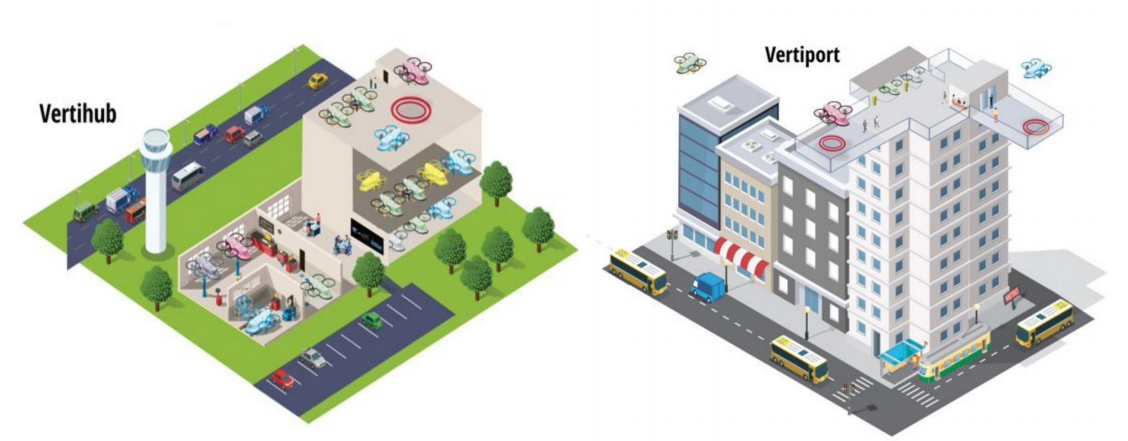
\includegraphics[width=0.98\columnwidth]{UAM-NFM/Figures/vert.PNG}
	\caption{Vertihub and vertiport depiction}
	\label{fig:uam_architecture}
\end{figure}


The UAM setting is unique as most flights will be on-demand and hence will require a controller that can \emph{react} to an unpredictable environment and provide guarantees of safety and liveness. Reactive synthesis~\cite{bloem2018graph} is a natural candidate to produce such controllers. A user (such as a regulatory body) can specify requirements in linear temporal logic for the operations of each vertihub and vertiport in the system. The task is to synthesize controllers for each vertihub and vertiport separately, guaranteeing that, together, the joint operation of the global system satisfies the conjunction of all specifications while still guaranteeing progress for the vehicles. In order to ensure that each controller does not impede the ability of other controllers to satisfy their requirements, we introduce a contract-based synthesis method which we formulate as a Generalized Reactivity(1) (GR(1))~\cite{bloem2012} synthesis problem that can be solved efficiently~\cite{wolff2013efficient,alur2016compositional}. Hence, our proposed solution architecture is scalable without sacrificing any safety or liveness guarantees. 


\subsection{Contributions}
This work is the first that considers a hierarchical, decentralized synthesis framework for UAM air traffic management. We use temporal logic for a formal representation of safety regulations and provably verify that these properties are satisfied across the global system. The contributions are as follows:

\begin{itemize}
	\item We design an architecture that allows a user (such as a regulatory body interested in guaranteeing safe operations) to specify safety requirements for the operations at each vertihub and vertiport. 
	\item The architecture allows the controller for each vertihub and vertiport to be synthesized separately, hence avoiding the state-space explosion of centralized synthesis. 
	\item We use contracts to guarantee that the joint interactions of all the individual controllers still satisfy all the safety requirements. Vehicles are guaranteed to still make progress towards their goals. 
	\item We provide high-fidelity simulations on large-volume projected UAM traffic data to showcase the applicability of our proposed architecture.
\end{itemize}

\subsection{Path to deployment}

Assessing the safety of an increasingly autonomous system relies on being able to bound the behavior and interactions of the components of the system as well as its interfaces with its operational environment. Performance-based regulation is employed in aviation to specify explicit properties that must be evinced by a component or element of the system (and/or operational environment) in order for the system safety claims to be met.  For example, 14 CFR \S 107.49 (d) states that: “If the small unmanned aircraft is powered, ensure that there is enough available power for the small unmanned aircraft system to operate for the intended operational time”.  This energy requirement forms a temporal logic constraint on the vehicle during its flight. The controller synthesis method for the vertihubs must adhere to this constraint in order to demonstrate compliance to 14 CFR \S 107.49.  The minimum violation guarantees provided by the presented synthesis process help to demonstrate that this regulation will be satisfied as much as possible throughout the flight process.  Thus, the guarantees provided by the synthesis method presented in this chapter may serve as a partial means of compliance to the regulation---supplemented with the generation of test and design analysis artifacts as well as operational procedures.

The presented synthesis framework provides a path to deployment of these increasingly autonomous systems in safety-critical contexts.  Air traffic management services, such as aircraft separation, may then be offered in a UAS Traffic Management (UTM) inspired framework, which interfaces with today’s traditional Air Traffic Management framework~\cite{PRKRJJ2016}. In this framework,  authority may be delegated by the FAA to provide select air traffic management services such as low-altitude weather information, congestion management, terrain avoidance, route planning, re-rerouting, separation management, and contingency management~\cite{MBYDLGMC2018,NCDDASC2018}.  One of the main attributes of the UTM system is that it does not require human operators to monitor every vehicle continuously, as in the traditional ATM system, thereby enabling increasingly autonomous realizations of specified air traffic management functions.  NASA has led UTM research over the past five years and is currently involved in the development and testing of a prototype UTM system with the FAA, in conjunction with numerous industry and public agency partners.  

The integration of the approach in this chapter into a UTM-like construct provides a path to deployment for UAM operations, as the provided safety guarantees will greatly enhance the assurance case for higher-risk operations currently not supported by UTM (e.g., operations in dense urban environments with UAS exceeding 55 lbs).


\section{Related work}

 Some preliminary work is being done in cooperative ATM for next generation air traffic management \cite{prevot2005co}, but this work considers a scheduled approach for large passenger aircraft and cannot handle management for on-demand flights. Similarly, work has been done on distributed control for ATM of small unmanned aerial systems (UAS) \cite{FSLLK2015}, but this work relies on cloud based architectures that do not currently satisfy strict aviation safety requirements.  Hybrid control approaches have been applied \cite{tomlin1996hybrid}, however scalability proves to be an issue.


With respect to the state-of-the-art, this is the first approach to
controller synthesis with safety guarantees for large-scale UAM ATM operations. Formally verified tools such as DAIDALUS~\cite{Daidalus} provide safety guarantees at lower levels of operations, however, they do not handle the fleet-level operations. The most similar approach to the one presented in this chapter is \emph{runtime enforcement}~\cite{Falcone10,Schneider00} of a specified property, in which a synthesized module detects and alters the behavior of the system in a way that maintains the desired property. An existing approach called shielding~\cite{BloemKKW15,KonighoferABHKT17} uses reactive synthesis and assumes that the shield has full knowledge and control of the whole system --- in this case the entire UAM system and the vehicles it handles. 

A technique for synthesizing quantitative shields for multi-agent systems in a fully centralized manner was presented in \cite{multiagentshield}. All these approaches rely on restrictive assumptions on runtime communication (e.g., full network coverage) and the extent of awareness and control authority of the shield (e.g., the shield can affect any agent in the network instantaneously). This requirement was relaxed in~\cite{bhnfm} where a local shield was synthesized for each sector with contracts between neighbors to guarantee global correctness. However, the approach was formulated only for specific safety properties (e.g., minimum-separation) and not more general properties such as liveness as is done here. We do not consider quantitative properties or optimality of behavior in this work, as the primary focus is the guarantee of specifications.

The work detailed in the following directly extends~\cite{bhnfm} by generalizing the class of allowable safety properties to any property in the GR(1)~\cite{bloem2012} fragment of linear temporal logic. Furthermore, the work in~\cite{bhnfm} was limited to very specific vehicle behaviors and could not handle take-off or landing requests. In this work, we introduce vertiport controllers that operate in the sector regions to additionally handle take-off and landing requests. The induced hierarchical structure allows for \emph{separation of concerns} between the vertihub and vertiport controllers. A decentralized, hierarchical approach for ATM was proposed in~\cite{6011668}, but unlike the setting in this chapter, it cannot handle temporal logic specifications. Hence, we are able to systematically synthesize controllers for ATM that can guarantee complex temporal requirements unlike conventional ATM approaches such as~\cite{6011668}. 
